\documentclass[11pt]{article}
\usepackage[english]{babel}
\usepackage[utf8]{inputenc}
\usepackage{amsmath,amsthm,amssymb,graphicx,pdfpages,lipsum,hyperref}
\usepackage[none]{hyphenat}
\setlength\parindent{0pt}
\usepackage[top=0.9in, left=0.9in, bottom=0.9in, right=0.9in]{geometry} 
\usepackage{natbib}
\usepackage{subfigure}
\usepackage{layouts}
\usepackage{caption}
\usepackage{graphicx}
\usepackage{booktabs}
\usepackage{float}


\def\*#1{\mathbf{#1}}

%%%%%%%%%%%%%%%%%%%%%%%%%%%%%%%%%%%%%%%%%%%%%%%%%%%%%%%%%%%%%%%%%%%

\title{\textbf{Spatiotemporal Dataset Analysis} \\ MAST30034: Assignment 1}
\author{Jason F. Suhartanto \\ 1086250}
\date{Semester 2, 2021.}

\begin{document}
\maketitle

\section{Synthetic Data Generation, Preprocessing, and Visualization}

Addressing the spatiotemporal data properties, we have these constant values to be used throughout the entire analysis:


\begin{enumerate}
    \item $N = 240$, the number of variables of the temporal sources. 
    \item $V = 441$, the number of variables of the spatial sources; where $x1 = 21$ and $x2 = 21$ is the shape of each two-dimensional spatial source.
    \item $NSRCS = 6$, the number of spatiotemporal sources.
\end{enumerate}

Additionally, a glossary of abbreviations is provided below for better understanding of the analysis.

\begin{enumerate}
    \item TC: Time Courses, the temporal source.
    \item SM: Spatial Maps, the spatial source.
    \item CM: Correlation Matrix.
    \item MSE: Mean Squared Error.
    \item LSR: Least Square Regression.
    \item RR: Ridge Regression
    \item LR: LASSO (Least Absolute Shrinkage and Selection Operator) Regression.
    \item PCR: Principal Component Regression.
\end{enumerate}

This analysis is performed using Python 3.9.

\subsection{Temporal Sources Generation: Time Courses ($\mathbf{TC}$)}

\begin{figure}[H]
    \begin{center}
       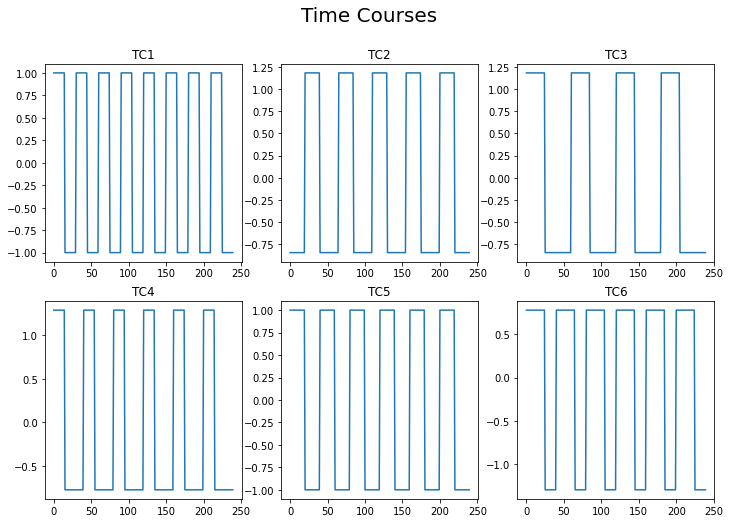
\includegraphics[width=0.9\textwidth]{../plots/1_1_TC}
      \caption{Time Courses $\mathbf{TC}$ generation from six sources.}
      \label{fig:time_courses}
    \end{center}
  \end{figure}

The temporal sources are generated from the provided onset arrival vector (AV), increment vector (IV), and duration of ones of six sources. $\mathbf{TC}$ matrix has size 240x6. Figure~\ref{fig:time_courses} shows the normalized $\mathbf{TC}$ accross six sources. Each column is standardized to have a mean of zero and unit variance.

We do not normalize by dividing it by l-2 norm because while the data is scaled to be between zero and one, the contribution of every source will depend on their scales which will cause a potential bias. Additionally, we are unable to infer if the data is already Gaussian, so standardization is preferred.

\subsection{Correlation Matrix Between TCs}

\begin{figure}[H]
    \begin{center}
       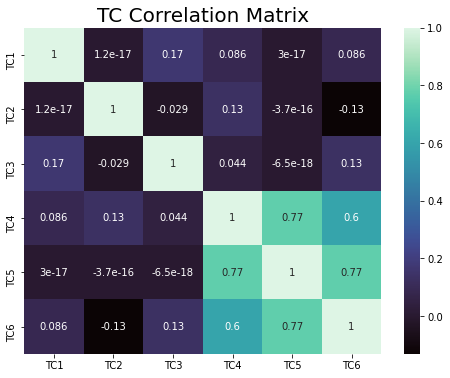
\includegraphics[width=0.6\textwidth]{../plots/1_2_correlationmatrix}
      \caption{Correlation Matrix (Pearson) between six Time Course (TC) sources.}
      \label{fig:TC_CM}
    \end{center}
  \end{figure}

  As of Figure~\ref{fig:TC_CM}, there are two pairs of TCs that have the highest correlation: TC4 and TC5 (0.77), and TC5 and TC6 (0.77). Additionally TC4 and TC6 have a correlation score of 0.6. The other TCs do not show a significant correlation with any of the other TCs.


\subsection{Spatial Sources Generation: Spatial Maps (SM)}

\begin{figure}[H]
    \begin{center}
       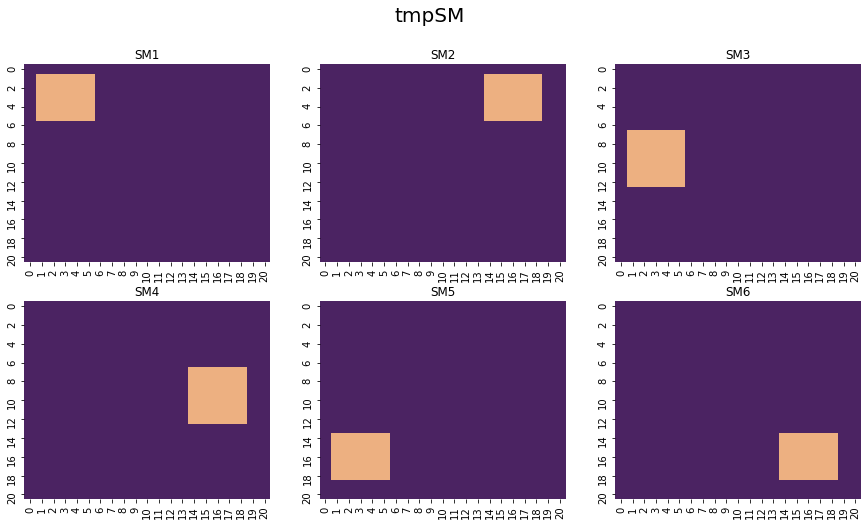
\includegraphics[width=0.9\textwidth]{../plots/1_3_a_SMs}
      \caption{Spatial Maps (SM) Generation from six sources.}
      \label{fig:sm_generation}
    \end{center}
  \end{figure}

For the spatial sources, the ones are visualized as the orange squares on the heatmaps, as shown in Figure~\ref{fig:sm_generation}. The ticks use Python indexing. To match the indexing in R in the assignment questions, the numbers are adjusted by one. E.g. for source 1, indices [2:6, 2:6] inclusive becomes indices [1:5, 1:5] inclusive in Python. The resulting $\mathbf{SM}$ matrix has size 6x441.

  \begin{figure}[H]
    \begin{center}
       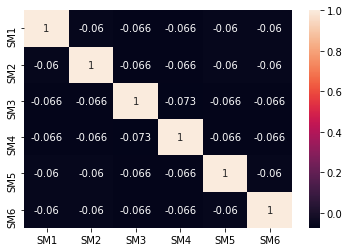
\includegraphics[width=0.6\textwidth]{../plots/1_3_b_SM_corr}
      \caption{Correlation matrix between six generated spatial sources.}
      \label{fig:sm_corr}
    \end{center}
  \end{figure}

As in Figure~\ref{fig:sm_corr}, the generated Spatial Maps (SM) sources do not have significant correlation between each other. However, correlation does not imply independence so we cannot say for sure that they are independent. Standardization for these spatial sources are not needed because each source already have a similar scale and mean.

\subsection{Noise Generation ($\mathbf{\Gamma_t}$ and $\mathbf{\Gamma_s}$)}

  \begin{figure}[H]
      \begin{center}
         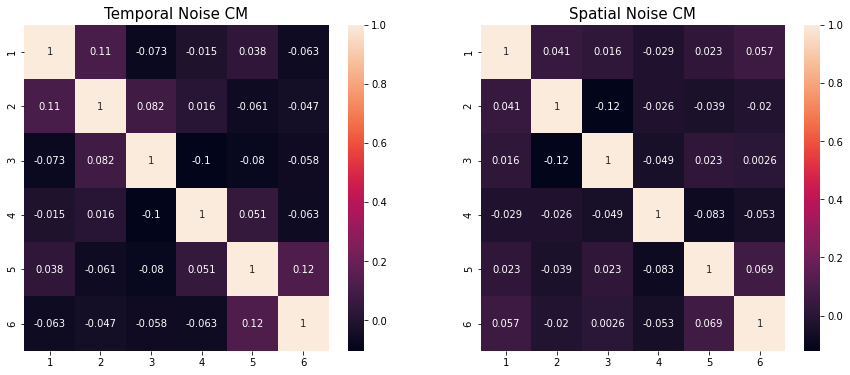
\includegraphics[width=0.85\textwidth]{../plots/1_4_temporal_and_spatial_noise_CM}
        \caption{Correlation matrix of generated temporal noises (left) and spatial noises (right).}
        \label{fig:noise_corr}
      \end{center}
    \end{figure}

The generated noise for temporal ($\mathbf{\Gamma_t}$) and spatial ($\mathbf{\Gamma_s}$) do not show a significant correlation with each other, as show in Figure~\ref{fig:noise_corr}. This is expected since they are generated randomly, and desirable because we do not want the noise to change the actual correlation information of the original data.
  
    \begin{figure}[H]
      \begin{center}
         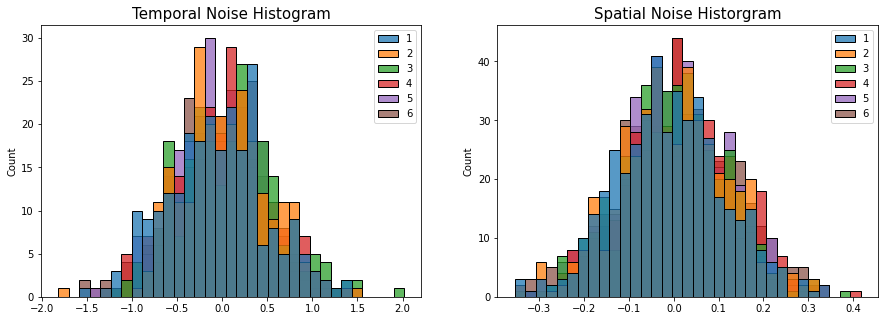
\includegraphics[width=0.9\textwidth]{../plots/1_4_temporal_and_spatial_noise_hist}
        \caption{Histograms showing distribution of values of temporal noises (left) and spatial noises (right).}
        \label{fig:noise_hist}
      \end{center}
    \end{figure}

The noise for each temporal and spatial source are shown to have a normal distribution, as in Figure~\ref{fig:noise_hist}. It can also be observed that they are both centered at the zero mean, and the distribution of the temporal noise is wider than the spatial noise because it has a higher standard deviation ($\sigma^2_t = 0.25$; $\sigma^2_s = 0.015$). Both distributions fulfill the mean and variance criteria.

    \begin{figure}[H]
        \begin{center}
           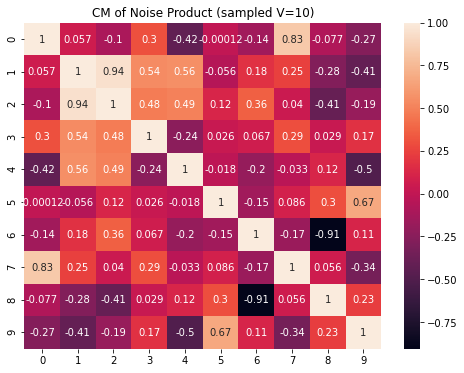
\includegraphics[width=0.6\textwidth]{../plots/1_4_noise_product_CM}
          \caption{Correlation matrix of noise product.}
          \label{fig:noiseprod_cm}
        \end{center}
      \end{figure}

Figure~\ref{fig:noiseprod_cm} shows the correlation of a sampled number of $V$ (out of 441 variables) of the Noise Product $\mathbf{\Gamma_t \Gamma_s}$. It is observed that some variables are highly correlated, both positively and negatively. 

\subsection{Synthetic Dataset Generation}

The synthetic spatiotemporal dataset $\mathbf{X}$ is created from the equation $\mathbf{X} = (\mathbf{TC} + \mathbf{\Gamma_t}) \times (\mathbf{SM} + \mathbf{\Gamma_s})$, and therefore has size 240x441. The matching matrix sizes allow $\mathbf{TC} \times \mathbf{\Gamma_s}$ and $\mathbf{\Gamma_t} \times \mathbf{SM}$ to exist. However if we use these products instead of the original equation, the information will be meaningless because of the product result of noise that is mostly centered at zero.

    \begin{figure}[H]
        \begin{center}
            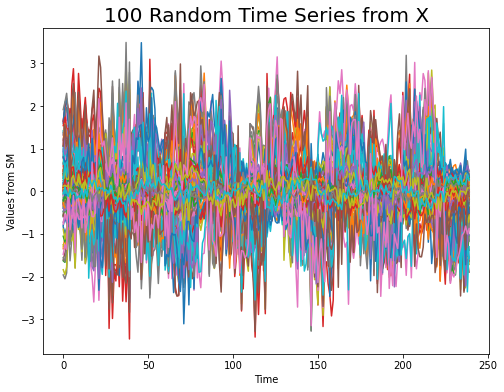
\includegraphics[width=0.5\textwidth]{../plots/1_5_100_random_time_series}
        \caption{100 randomly selected time series from the spatiotemporal synthetic dataset ($\mathbf{X}$) before standardization.}
        \label{fig:100_timeseries}
        \end{center}
    \end{figure}

    \begin{figure}[H]
        \begin{center}
            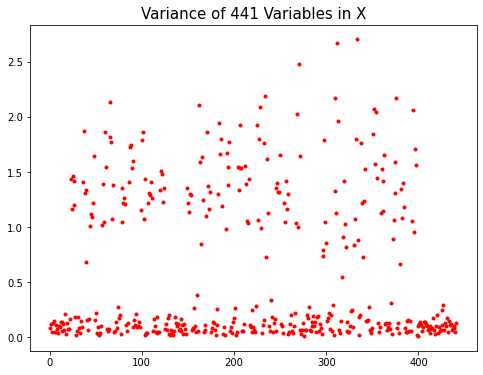
\includegraphics[width=0.5\textwidth]{../plots/1_5_variance_distribution}
        \caption{Variance distribution of the 441 variables from the spatiotemporal synthetic dataset $\mathbf{X}$ before standardization.}
        \label{fig:vardist_X}
        \end{center}
    \end{figure}

Randomly selected samples of time-series from a non-standardized $\mathbf{X}$ are shown in Figure~\ref{fig:100_timeseries}, which shows behaviour of the spatial data across 241 time units. We can also observe inconsistent variances across 441 variables, as shown in Figure~\ref{fig:vardist_X}, as some variables have variance close to zero, but also many have high variances of more than 2.0. Observing these two plots, $\mathbf{X}$ needs to be standardized.


\section{Data Analysis, Results Visualization, Performance Metrics}

\subsection{Least Square Regression (LSR)}
\label{section:lsr}

    \begin{figure}[H]
        \begin{center}
            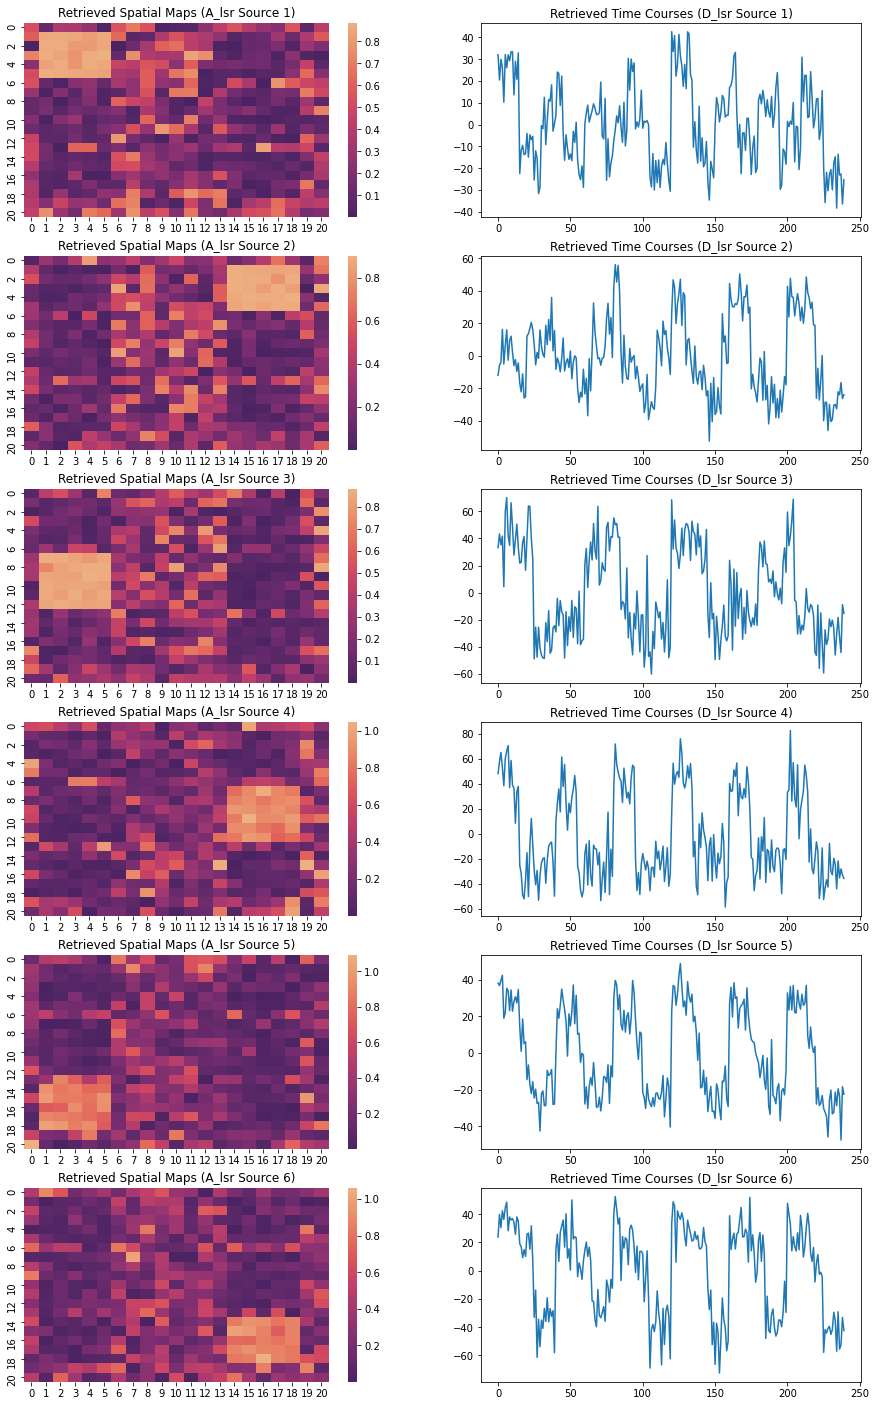
\includegraphics[width=0.7\textwidth]{../plots/2_1_Alsr_Dlsr}
        \caption{Retrieved spatial sources (left column) and temporal sources (right column) by least square regression (LSR).}
        \label{fig:lsr_all}
        \end{center}
    \end{figure}

The synthetic spatiotemporal dataset $\mathbf{X}$ follows a linear regression model $\mathbf{X} = \mathbf{DA} + \mathbf{E}$. Using the least squares method:

\begin{enumerate}
    \item $ \*A_{LSR} = (\*D^\top \*D)^{-1} \*D^\top \*X $, where $ \*D = \*{TC}$.
    \item $ \*D_{LSR} = \*X \*A^\top_{LSR}$.
\end{enumerate}

From this LSR parameters estimation, these correlation vectors are obtained:

\begin{enumerate}
    \item $\mathbf{c}_{TLSR}$, the absolute correlation vector between $\*{TC}$ and $\*D_{LSR}$.
    \item $\mathbf{c}_{SLSR}$, the absolute correlation vector between $\*{SM}$ and $\*D_{LSR}$.
\end{enumerate}

The retrieved spatial and temporal sources across six sources are shown in Figure~\ref{fig:lsr_all}.

    \begin{figure}[H]
        \begin{center}
            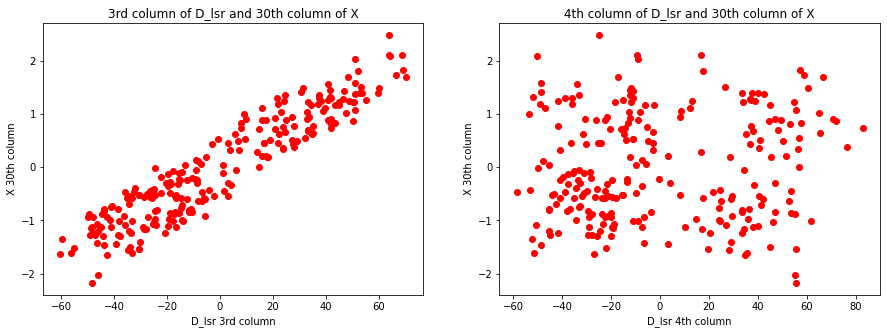
\includegraphics[width=0.9\textwidth]{../plots/2_1_Dlsr_vs_X_linear}
        \caption{These scatter plots investigates linear relationships between slices of the $D_{LSR}$ estimates and $X$.}
        \label{fig:dlrs_linear}
        \end{center}
    \end{figure}

In Figure~\ref{fig:dlrs_linear}, we can see that some columns in $\*X$ and columns in $\*D_{LSR}$ have a linear relationship. E.g., the 3rd column of $\*D_{LSR}$ is constructed by the 30th column of $\*X$ when estimating with $\*X \*A^\top_{LSR}$. However, this is not the case of the following 4th column in $\*D_{LSR}$ because they are not estimated using the same 30th column variable in $\*X$.

\subsection{Ridge Regression (RR)}
\label{sec:rrestimate}

The Ridge Regression (RR) parameters are estimated by:

\begin{enumerate}
    \item $ \*A_{RR} = (\*D^\top \*D + \tilde{\lambda} \*I )^{-1} \*D^\top \*X $, where $ \*D = \*{TC}$ and $\tilde{\lambda} = \lambda V$.
    \item $ \*D_{RR} = \*X \*A^\top_{RR}$.
    
\end{enumerate}

We set $\lambda$ = 0.2 for this RR estimation using a check and guess method. From this RR parameters estimation, these correlation vectors are obtained:

\begin{enumerate}
    \item $\mathbf{c}_{TRR}$, the absolute correlation vector between $\*{TC}$ and $\*D_{RR}$.
    \item $\mathbf{c}_{SRR}$, the absolute correlation vector between $\*{SM}$ and $\*D_{RR}$.
\end{enumerate}

    \begin{figure}[H]
        \begin{center}
            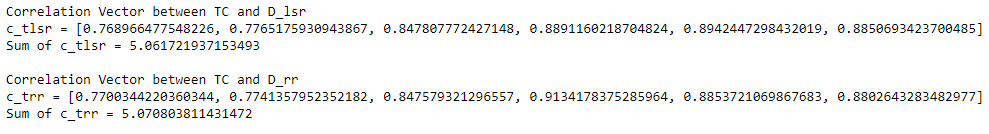
\includegraphics[width=0.9\textwidth]{../plots/2_2_ctlsr_ctrr_sums}
        \caption{Comparison of sums of correlation vectors from Least Square Regression (LSR) and Ridge Regression (RR).}
        \label{fig:corrvec_lrs_rr}
        \end{center}
    \end{figure}



As in Figure~\ref{fig:corrvec_lrs_rr}, we found that the $\sum \mathbf{c}_{TRR}$ (5.0708) to be higher than $\sum \mathbf{c}_{TLSR}$ (5.0617). Therefore we have selected a good value of $\lambda$ for the RR estimation, which is 0.2.

    \begin{figure}[H]
        \begin{center}
            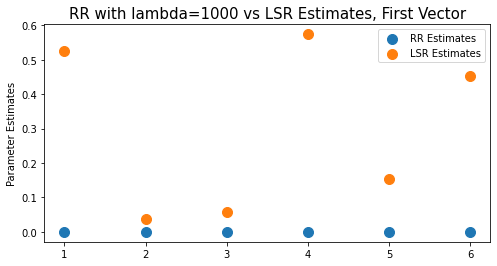
\includegraphics[width=0.7\textwidth]{../plots/2_2_rr1000_vs_lsr}
        \caption{First vector from $\*{A_{RR}}$ when $\lambda=1000$, compared with the first vector from $\*{A_{LSR}}$.}
        \label{fig:lrs_vs_rr_1000}
        \end{center}
    \end{figure}

When $\lambda$ is set to be 1000, we found all estimated RR parameters to shrink towards zero, as expected. This is shown in Figure~\ref{fig:lrs_vs_rr_1000}, and compared with the estimated parameters from LSR in Section \ref{section:lsr}.

\subsection{Finding $\rho$ for LASSO Regression (LR)}
\label{section:findp}

    \begin{figure}[H]
        \begin{center}
            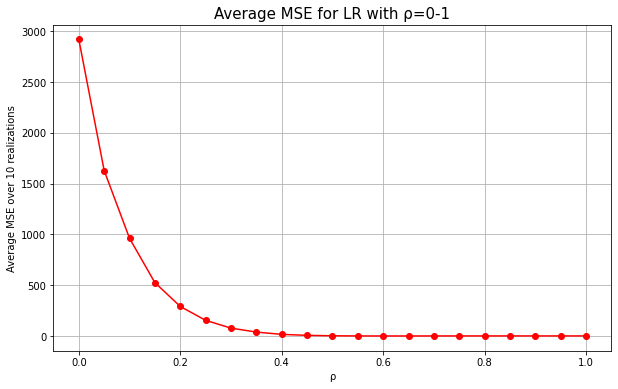
\includegraphics[width=0.7\textwidth]{../plots/2_3_MSE_vs_rho_LR}
        \caption{Average Mean Square Error (MSE) of LR estimates for different $\rho$ values.}
        \label{fig:find_rho}
        \end{center}
    \end{figure}

Testing different $\rho$ values for LR estimation on different realizations, we found the optimal $\rho$ value to be 0.60, as seen in Figure~\ref{fig:find_rho}. Setting $\rho = 0.60$ gives the lowest average Mean Squared Error (MSE) of 0.4575, and therefore we select this value for the regression in the following section. The MSE is also observed to start increasing again for $\rho$ greater than 0.60.

\subsection{LASSO Regression (LR) Estimation}

LASSO Regression is performed following the provided pseudocode and setting $\rho = 0.60$ as in Section~\ref{section:findp}. From this LR parameters estimation, these correlation vectors are obtained:

\begin{enumerate}
    \item $\mathbf{c}_{TLR}$, the absolute correlation vector between $\*{TC}$ and $\*D_{LR}$.
    \item $\mathbf{c}_{SLR}$, the absolute correlation vector between $\*{SM}$ and $\*D_{LR}$.
\end{enumerate}

    \begin{figure}[H]
        \begin{center}
            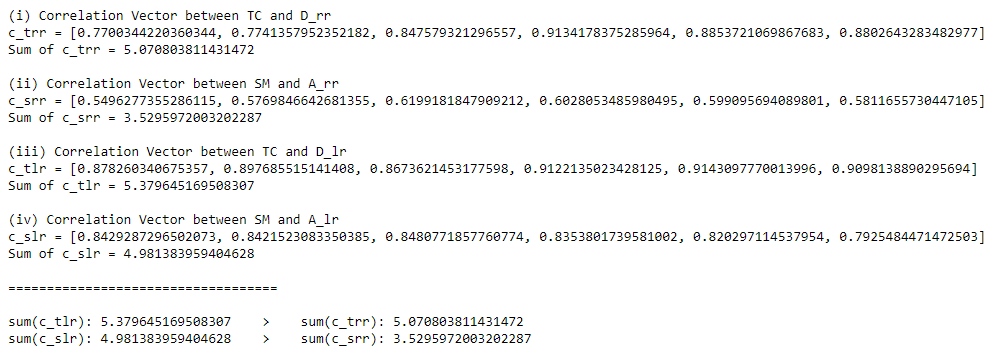
\includegraphics[width=0.95\textwidth]{../plots/2_4_CorrVector_RRvsLR}
        \caption{Correlation vectors comparison between estimates of Ridge Regression (RR) and LASSO Regression (LR).}
        \label{fig:corrvec_lr_rr}
        \end{center}
    \end{figure}

We found that $\sum \mathbf{c}_{TLR}$ (5.3796) to be higher than $\sum \mathbf{c}_{TRR}$ (5.0708), and $\sum \mathbf{c}_{SLR}$ (4.9814) to be higher than $\sum \mathbf{c}_{SRR}$ (3.5296). Therefore we have selected a good value of $\rho$ for the LR estimation, which is 0.6. 

    \begin{figure}[H]
        \begin{center}
            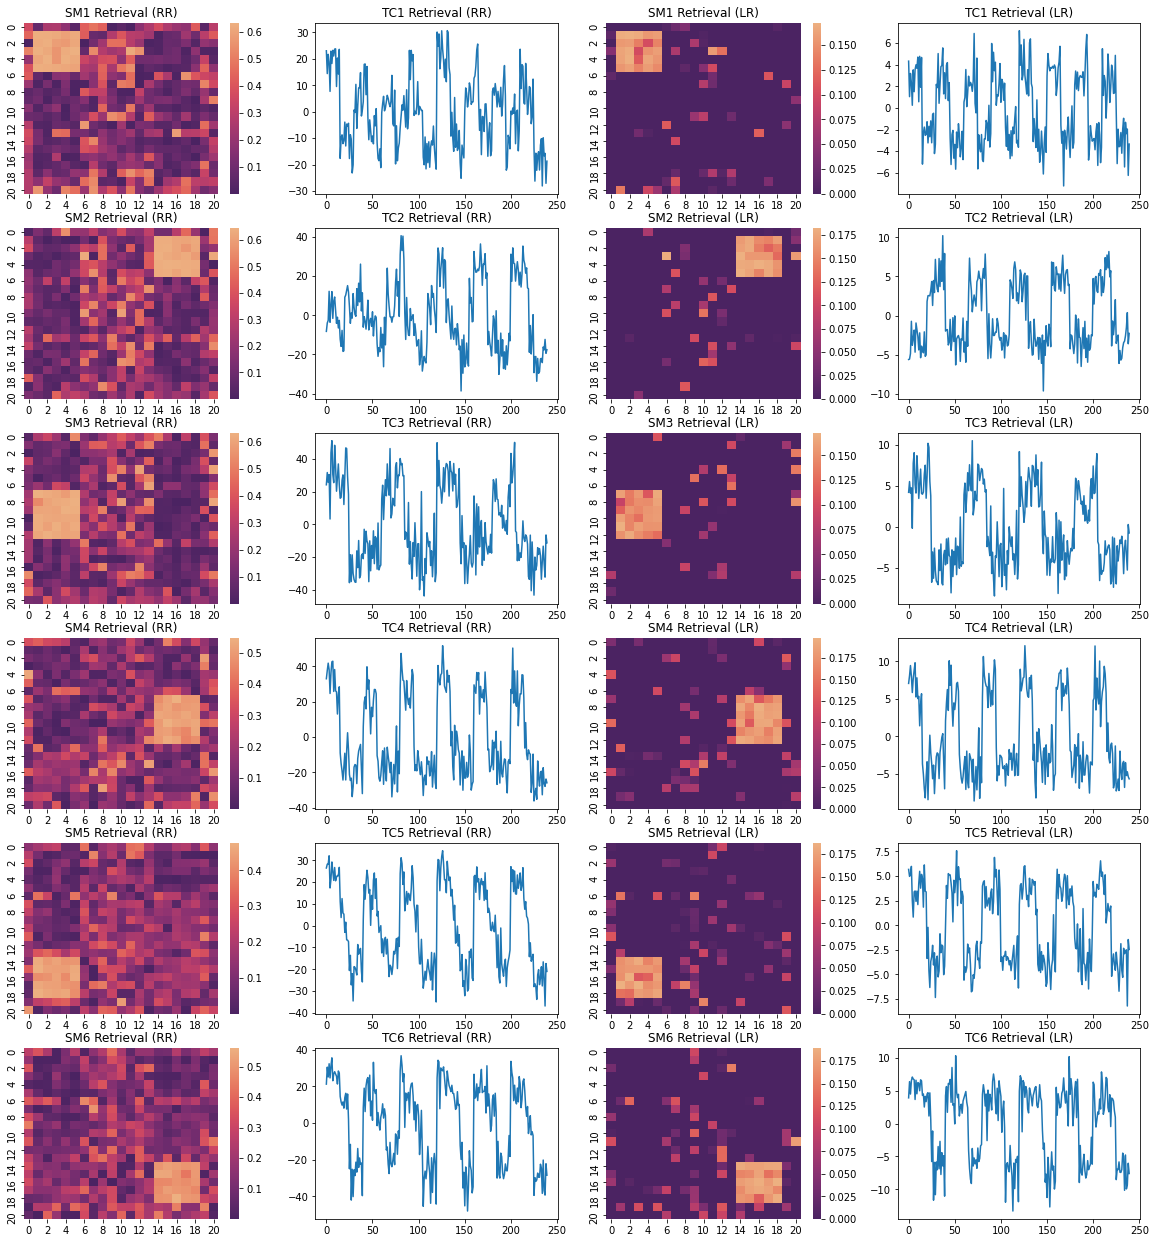
\includegraphics[width=0.95\textwidth]{../plots/2_4_RR_vs_LR_all}
        \caption{Retrievals comparison of Ridge Regression (left half) and LASSO Regression (right half).}
        \label{fig:rr_vs_lr_all}
        \end{center}
    \end{figure}

The comparison of $\*D$ and $\*A$ estimates for LR and RR are shown in Figure~\ref{fig:rr_vs_lr_all}. We can see that LR performs exceptionally better than RR, as RR gives more false positives. One reason is because LR works better for multicollinearity (MC). Another reason is because LR is able to remove variables that have very low relevance, rather than just shrinking it towards zero, and therefore reduces overfitting better. In this case, we can infer that the data carries noise.

\subsection{Principal Component Regression (PCR)}

Estimating the Principal Components (PC) of the TCs is performed by calling the Singular Value Decomposition\footnote{Retrieved from \href{https://numpy.org/doc/stable/reference/generated/numpy.linalg.svd.html}{https://numpy.org/doc/stable/reference/generated/numpy.linalg.svd.html}, accessed on September 5, 2021.} function from NumPy in Python. The regressors are denoted as $\*Z$.

    \begin{figure}[H]
        \begin{center}
            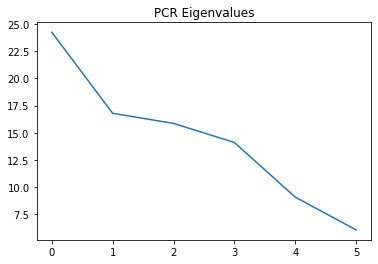
\includegraphics[width=0.7\textwidth]{../plots/2_5_eigenvalues_min}
        \caption{Eigenvalues from the Principal Component Regression.}
        \label{fig:pcr_eigenvals}
        \end{center}
    \end{figure}

From Figure~\ref{fig:pcr_eigenvals}, we see that the eigenvalue is smallest for the sixth Principal Component (PC). 

    \begin{figure}[H]
        \begin{center}
            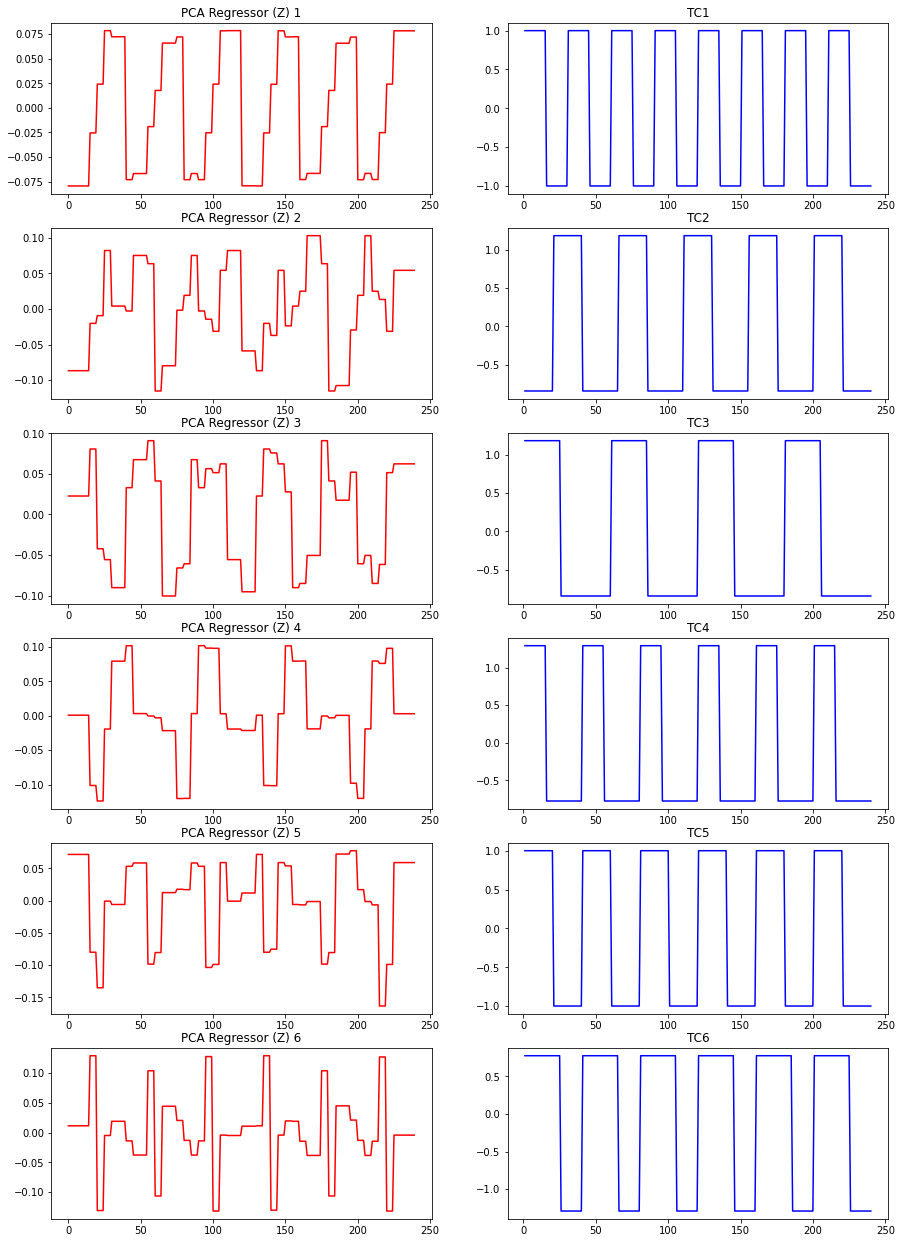
\includegraphics[width=0.8\textwidth]{../plots/2_5_PCAreg_vs_TC}
        \caption{Regressors from PCR (left column) and the actual temporal sources (right column).}
        \label{fig:z_vs_tc}
        \end{center}
    \end{figure}

The regressors $\*Z$ are compared with its actual TC source in Figure~\ref{fig:z_vs_tc}. We can also see that the PCs have a deteriorated shape and the shape of the TCs are lost. This is because the Principal Components are linear combinations of the TCs. Applying PCA before the regression will remove variability of TC without knowledge which are the most significant.

    \begin{figure}[H]
        \begin{center}
            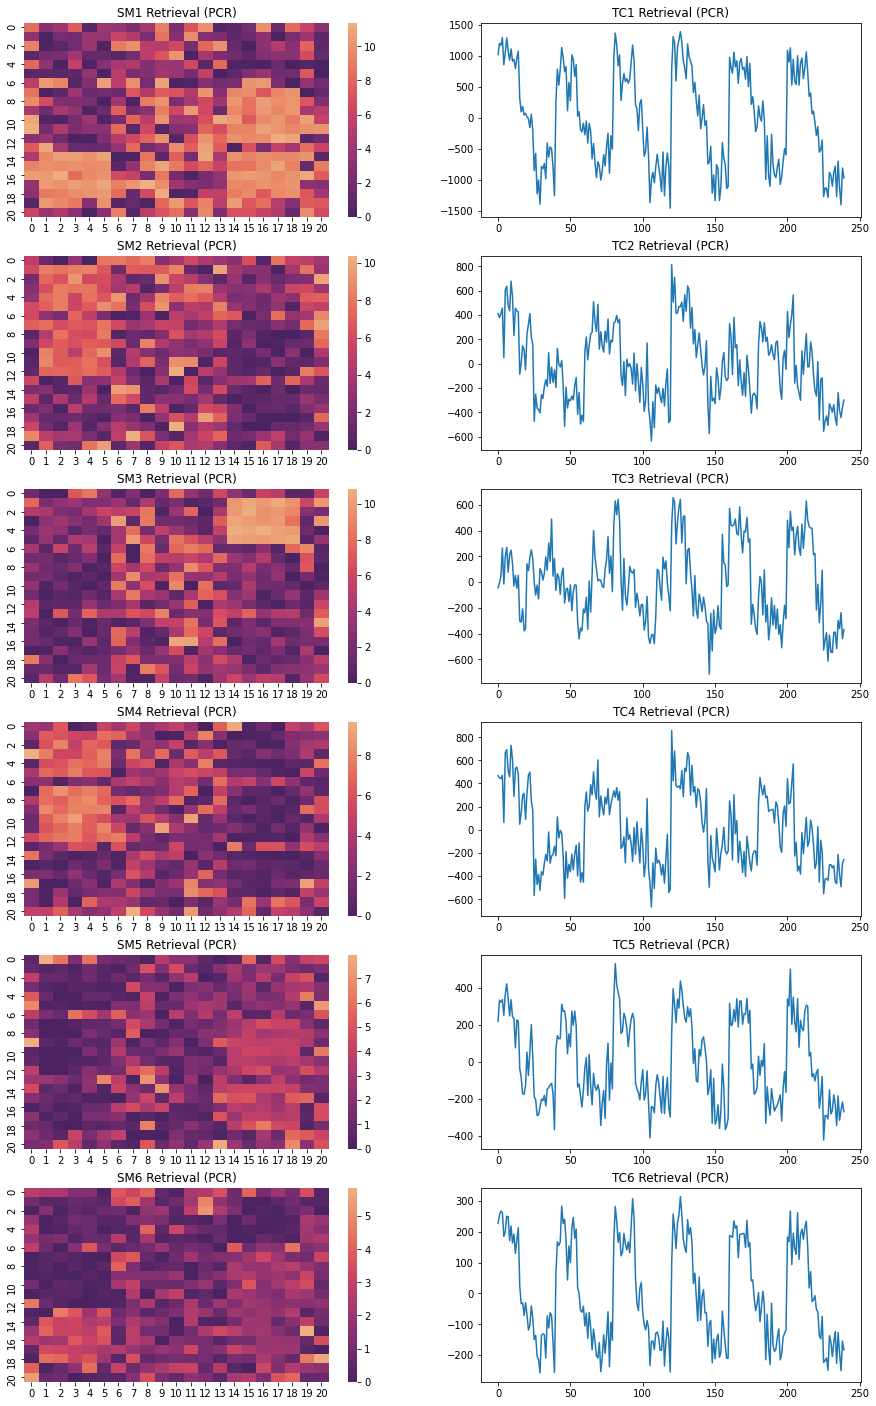
\includegraphics[width=0.8\textwidth]{../plots/2_5_PCR_retrievals}
        \caption{Spatial (left column) and Temporal (right column) retrievals of Principal Component Regression.}
        \label{fig:pcr_retrievals}
        \end{center}
    \end{figure}

For the Principal Component Regression (PCR), a LASSO Regression is performed on $\*X$ using $\*Z$ as the regressors, instead of regressing the dependent variables directly on the explanatory variables. A $\rho$ value of 0.001 is used. The retrievals, $\*D_{PCR}$ and $\*A_{PCR}$, are shown in Figure~\ref{fig:pcr_retrievals}. This result is inferior and shows a poorer estimate compared to LSR, RR, and LR. This is expected because on PCR we performed dimensionality reduction on TC to get $\*Z$ as the regressors $\*D$, whereas on LSR, RR, and LR, the regressors are assumed to be known as we set $\*D = \*{TC}$, and therefore keeping a complete information. Applying PCA only makes sense if we want to simplify the data's dimensionality, not to obtain better accuracy.

\end{document}